\documentclass{article}

\usepackage{amsfonts}
\usepackage{amsmath}
\usepackage{graphicx}


\setlength\parindent{18pt}

\begin{document}

1) Beck excercise 1.1. Show that $||\cdot||_p$ for $p=\frac{1}{2}$ is not a norm.

\[||x||_p = (x_1^p + x_2^p + ... + x_n^p)^{\frac{1}{p}}\]

So
\[||x||_\frac{1}{2} = (\sqrt[2]{x_1} + \sqrt[2]{x_2} + ... + \sqrt[2]{x_n})^2\]

It must satisfy:
1) non-negativity
2) positive homogeneity
3) triangle inequality


The triangle inequality does not hold.

Take:
\[r_1 = (1, 0), r_2 = (0, 1)\]

If we plug this in to $||x||_\frac{1}{2}$, we get:

\[||r_1 + r_2||_\frac{1}{2} = (\sqrt[2]{1} + \sqrt[2]{1})^2 = (1 + 1)^2 = 2^2 = 4\]

But:

\[||r_1||_\frac{1}{2} + ||r_2||_\frac{1}{2}
= (\sqrt[2]{1})^2 + (\sqrt[2]{1})^2 = 1 + 1 = 2\]


So, the statement that $||r_1 + r_2||_\frac{1}{2}
\leq ||r_1||_\frac{1}{2} + ||r_2||_\frac{1}{2}$ is false
and thus the triangle inequality is false, which means that
$||\cdot||_\frac{1}{2}$ is not a norm.



2) Let $x \in \mathbb{R}^n, n \in \mathbb{Z}$. Show that:

\indent \indent i)
\[||x||_\infty \leq ||x||_2 \leq \sqrt[2]{n}||x||_\infty\]

\[||x||_\infty = \max\limits_{1 \leq i \leq n} (x_i)\]

Since $\sqrt[2]{max^2+n^2} \iff  \sqrt[2]{||x||_\infty+n^2}$
is at least as big as $max$ $\forall n \in \mathbb{R}$,
then $||x||_\infty \leq ||x||_2$.


\[||x||_2 \leq \sqrt[2]{n}||x||_\infty\]
\[\iff ||x||^2_2 \leq n||x||^2_\infty\]
\[\iff ||x||_2 = x_1^2 + x_2^2 + ... + x_n^2
\leq n*\max\limits_{1\leq i \leq n} (x_i)^2\]

Well, since the only way these can be equal is if all
the entries of the vector are the same
(aka they're all $max$, so you end up with $n$ of their squares being summed),
and any other option results in $||x||^2_2|| < n||x||^2_\infty$
(since you have less than $n$ $max$ entries in your vector),
then $||x||^2_2 \leq n||x||^2_\infty \iff |x||_2 \leq \sqrt[2]{n}||x||_\infty$.


\indent \indent ii)
\[\frac{1}{\sqrt[2]{n}}||x||_1 \leq ||x||_2 \leq ||x||_1\]

\[\frac{1}{\sqrt[2]{n}}||x||_1 \leq ||x||_2 \leq ||x||_1\]
\[\iff \frac{1}{\sqrt[2]{n}}(|x_1| + |x_2| + ... + |x_n|)
\leq \sqrt[2]{x_1^2 + x_2^2 + ... + x_n^2}
\leq (|x_1| + |x_2| + ... + |x_n|)\]
\[\iff \frac{1}{n}(|x_1| + |x_2| + ... + |x_n|)^2
\leq (x_1^2 + x_2^2 + ... + x_n^2)
\leq (|x_1| + |x_2| + ... + |x_n|)^2\]

\[(x_1^2 + x_2^2 + ... + x_n^2)
\leq (|x_1| + |x_2| + ... + |x_n|)^2\]

is relatively obvious since the square of
several numbers will always be greater than or
equal to the sum of the squares of them individually
(you can think about the numbers as variables in a polynomial for instance).

\[\frac{1}{n}(|x_1| + |x_2| + ... + |x_n|)^2
\leq (x_1^2 + x_2^2 + ... + x_n^2)\]

is less obvious, but it makes sense if you consider that it is
effectively taking the average of the numbers multiplied together.
And the average value of a set of numbers being squared would
always be less than or equal to the sum of them squared individually.

For example, let $n$ be the maximum value in $x$.
You end up with $\frac{1}{n}(n*n)^2 \leq n*n^2 \iff \frac{n^4}{n} \leq n^3 \iff n^3 \leq n^3$.
In the case where it is not all of the same value (aka $max$), then
$\frac{1}{n}(|x_1| + |x_2| + ... + |x_n|)^2
\leq (x_1^2 + x_2^2 + ... + x_n^2)
\iff \frac{1}{\sqrt[2]{n}}||x||_1 \leq ||x||_2$.


3) Beck Excercises 1.8 and 1.9. Suppose that
$\mathbb{R}^m$ and $\mathbb{R}^n$ are equipped
with norms $||\cdot||_b$ and $||\cdot||_a$, respectively.

\[||A||_{a,b} = \max\limits_{x} \{||Ax||_b : ||x||_a \leq 1\}\]


\indent \indent i)
Show that the induced norm $||\cdot||_{a,b}$
can be computed by the formula

\[||A||_{a,b} = \max\limits_{x} \{||Ax||_b : ||x||_a = 1\}\]

Since $||x||_a = 0 \implies ||x||_a \leq 0$, it is clear that this is a valid way of computing $||A||_{a,b}$.


\indent \indent ii) Also show that

\[||A||_{a,b} = \max\limits_{x \neq 0} \frac{||Ax||_b}{||x||_a}\]


Since you are computing the quotient of $|Ax||_b$ and $||x||_a$,
in the case that $||x||_a > 1$,
the value will be lower and will not become the result of the $max$.
So in reality this implementation will end up choosing $||x||_a \leq 1$.


4) Beck Excercise 1.13. Let $A \in \mathbb{R}^{m \times n}$. Show that

\indent \indent i) $||A|| = ||A^{T}||$ where $||\cdot||$ is the spectral norm.

Since it is computing $(A^{T}A)$ and then taking the largest singular value,
whether or not you pass in the transpose of A or A
doesn't matter since the singular values will always
be the same for the resulting square matrix.


\indent \indent ii) $||A||^2_F = \sum_{i = 1}^{n} \lambda_i(A^{T}A)$

\[||A||^2_F = \sum_{i = 1}^{m}\sum_{j = 1}^{n} A^2_{ij}\]

Since you are summing up all of the entries of the matrix squared,
then it makes sense that it is equivalent to the sum of the
squared matrix (using A times its transpose)
scaled by the eigenvalue of that column
(since you are scaling by the amount that you would get
from summing up the column's entries).


5) Beck Excercise 1.14. Let $A \in \mathbb{R}^{m \times n}$
be a symmetric matrix. Show that

\[\lambda_{max}(A) = \max\limits_{x} \{x^{T}Ax: ||x||^2 = 1\}\]

This makes sense since you are taking $x$, applying $A$ onto it,
and then squashing it down into $\mathbb{R}$ without scaling it
(we aren't scaling it since $||x||^2 = 1$).
So you are essentially compressing the scaling from $A$ onto the real numbers.
So this is a valid way to get the maximum eigenvalue for the matrix since
you are computing the maximum scaling.


6) Taylor's Theorem.

\indent \indent i) Find the second-order Taylor approximation for $f(x) = sin(x)$
about the point $x = \frac{\pi}{2}$. Sketch a plot of $f(x)$ and the approximation.

\[f(\frac{\pi}{2}) = 1\]
\[f'(x) = cos(x)\]
\[f'(\frac{\pi}{2}) = 0\]
\[f''(x) = -sin(x)\]
\[f''(\frac{\pi}{2}) = -1\]

\[f(x) \simeq 1 - \frac{1}{2}(x - \frac{\pi}{2})^2\]


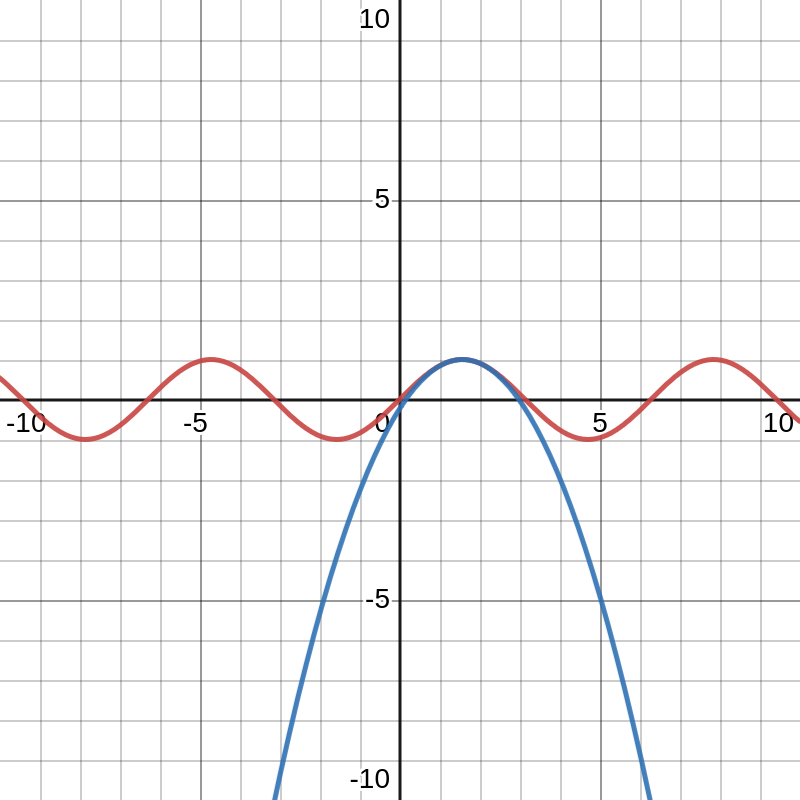
\includegraphics[width=\linewidth]{sinx_taylor_polynomial}



\indent \indent ii) Find the second-order Taylor approximation for

\[g(x_1, x_2) = 3 + e^{x_1} - e^{2x_2}\]

about the origin. Sketch a plot of $g(x_1, x_2)$ and the approximation.


\[g(0, 0) = 3\]
\[g_{x_1} = e^{x_1}\]
\[g_{x_1}(0, 0) = 1\]
\[g_{x_1 x_1} = e^{x_1}\]
\[g_{x_1 x_1}(0, 0) = 1\]
\[g_{x_1 x_2} = 0\]
\[g_{x_1 x_2}(0, 0) = 0\]
\[g_{x_2} = -2e^{2x_2}\]
\[g_{x_2}(0, 0) = -2\]
\[g_{x_2 x_2} = -4e^{2x_2}\]
\[g_{x_2 x_2}(0, 0) = -4\]


\[f(x_1, x_2) \simeq 3 + x_1 -2x_2 + \frac{1}{2}x_1^2 -2x_2^2\]


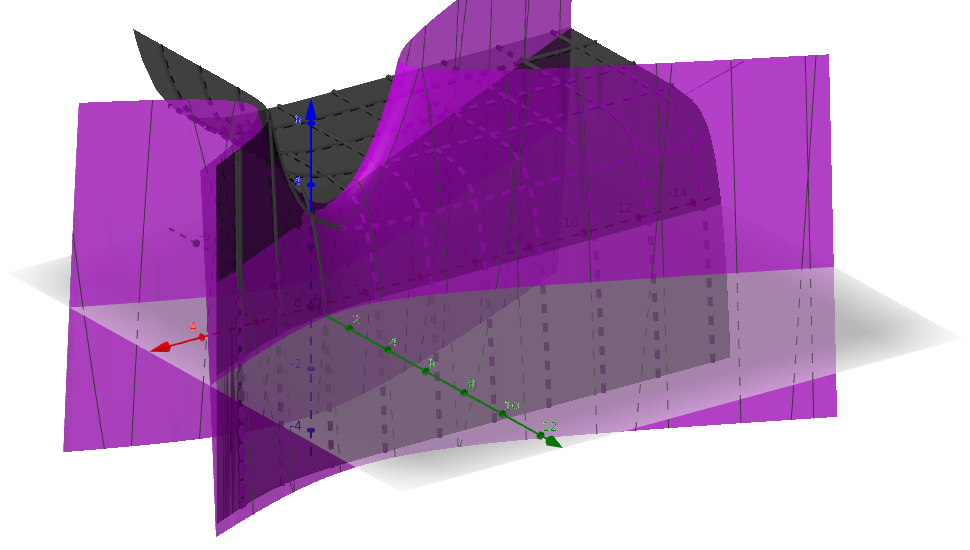
\includegraphics[width=\linewidth]{2d_taylor_approximation}



\end{document}
